\documentclass[aps,twocolumn,secnumarabic,balancelastpage,amsmath,amssymb,nofootinbib]{revtex4-1}

\usepackage{color}         % produces boxes or entire pages with colored backgrounds
\usepackage{graphics}      % standard graphics specifications
\usepackage[pdftex]{graphicx}      % alternative graphics specifications
\usepackage{epsf}          % old package handles encapsulated post script issues
\usepackage{bm}            % special 'bold-math' package
%\usepackage{asymptote}     % For typesetting of mathematical illustrations
\usepackage{thumbpdf}
%\usepackage{algorithm2e}

\begin{document}

\title{Blicycle: A Bicycle for the Blind}
\author{Steve Levine}
\date{\today}
\affiliation{Principles and Practice of Assistive Technology (6.S196) Final Report}

\maketitle

\section{Introduction}
We worked on developing blicycle - a bicycle for the blind. Blicycle is designed to be ridden in the closed, controlled environment of an outdoor track and incorporates a number of electronic, software, and mechanical modifications to an existing bicycle to make it accessible to the blind. We use computer vision to localize the bike with respect to the track, determine a desired steering angle for blicycle using this information, and communicate turning instructions to the rider using a vibrating handlebar interface. 

This project began with a contextual inquiry of our client, Brian, for whom we would design blicycle. After meeting with him and discussing his preferences and constraints, we began designing and prototyping a number of ideas for blicycle. We iterated on a number of different design ideas and met with Brian over the course of the semester for idea generation and user testing. By the end of the semester, in addition to completing a working prototype, we also learned a great deal about designing assistive technology. In the future, we would like to work more on this project in order to increase its robustness and reduce its chance of abandonment. 

\section{Contextual Inquiry and Task Analysis}
At the beginning of the semester, we met with Brian and began a contextual inquiry process. Brian is a 55-year old man who has been completely blind since the age of 11. He is currently the Director of Computer Training Services at the Carroll Center for the Blind, and is hence very familiar with assistive technologies. Additionally, Brian has an extremely acute ear - for example, he can easily identify the architecture of a room simply by its reverberation. Brian has full kinesthetic and tactile abilities. He also knows how to ride a bicycle. In fact, shortly after he became blind, Brian could go riding with his brothers and stay at the midpoint between them based on their whistling.

Brian informed us that, in the blind community, exercise is a formidable challenge. While a sighted person can easily go for a quick jog around town, the same task presents considerable difficulty for a blind person who, for example, may need to memorize how many streets to pass before taking appropriate turns. Additionally, detecting obstacles becomes an issue since traditional methods used by the blind, such as canes, are not effective when used while running at the aerobic speeds required for exercise. For these reasons, outdoor exercise is often accomplished with sighted people. An example of this is tandem bicycle riding, in which a sighted person sits in the front seat of the bicycle to navigate and watch for obstacles, and a blind individual sits in the back seat and pedals. While effective, this manner of exercise requires extensive coordination beforehand. Impromptu exercise - such as going out on a casual bike ride or jog - is a functional difficulty for the blind.

As such, Brian desired a bicycle or other means of exercise that would allow him to get exercise in the great outdoors while at the same time requiring assistance from no other people. Brian would ideally take his bicycle from storage at the Perkins School for the Blind's outdoor track (where he wishes to ride after work every day), and then go for a ride around the track after making sure it is not already in use. This would allow Brian to exercise outdoors independently, on his own schedule, without the help of anyone else, and without the need to plan far in advance.

Therefore, with exercise as his primary motivation, Brian requested us to design a technology to meet his constraints. Brian preferred biking over other means of outdoor exercise, and thus blicycle was born.

We outlined a series of qualitative and quantitative success metrics by which we could measure the effectiveness of blicycle - please see Figure \ref{fig:SuccessMetrics}. These metrics also guided many of our design choices, which we will describe shortly.

\begin{figure}
\begin{tabular}{| c | c |}
\hline
Success Metric & Score Range \\ \hline \hline
How aesthetic is the device? Conspicuous? & 0 - 10 \\ \hline
How comfortable is the device? & 0 - 10 \\ \hline
How safe does Brian feel with device? & 0 - 10 \\ \hline
How distracting / annoying is the device? & 0 - 10 \\ \hline \hline
How many laps can Brian complete? & 0 - 10 \\ \hline
How much time required to organize ride? & 0 - 10 \\ \hline
How many people required to be around? & 0 - 10 \\ \hline
How straight can Brian ride? Stays within \\ how many feet of center? & 3-20+ \\ \hline
How fast can Brian safely ride? & 0 - 15mph \\ \hline
\end{tabular}
\caption{Qualitative and quantitative success metrics.}
\label{fig:SuccessMetrics}
\end{figure}


\section{Design Process}
In designing blicycle, many of our design choices were motivated by the constraints implied by Brian's disability and the context of the situation. For example, one recurring consideration of this project is safety. Since riding a bicycle is inherently dangerous, we considered safety factors at every point in both the mechanical and software design of our project.

We decided to divide blicycle into three parts: 1.) Navigation, or determining when and how the bike should be steered, 2.) Obstacle Detection, for avoiding collisions, and 3.) User Interface, or communicating information about the previous two points to the rider. Each of these areas will be discussed in the following sections, along with corresponding design constraints imposed by Brian's preferences and functional abilities.

\begin{figure}
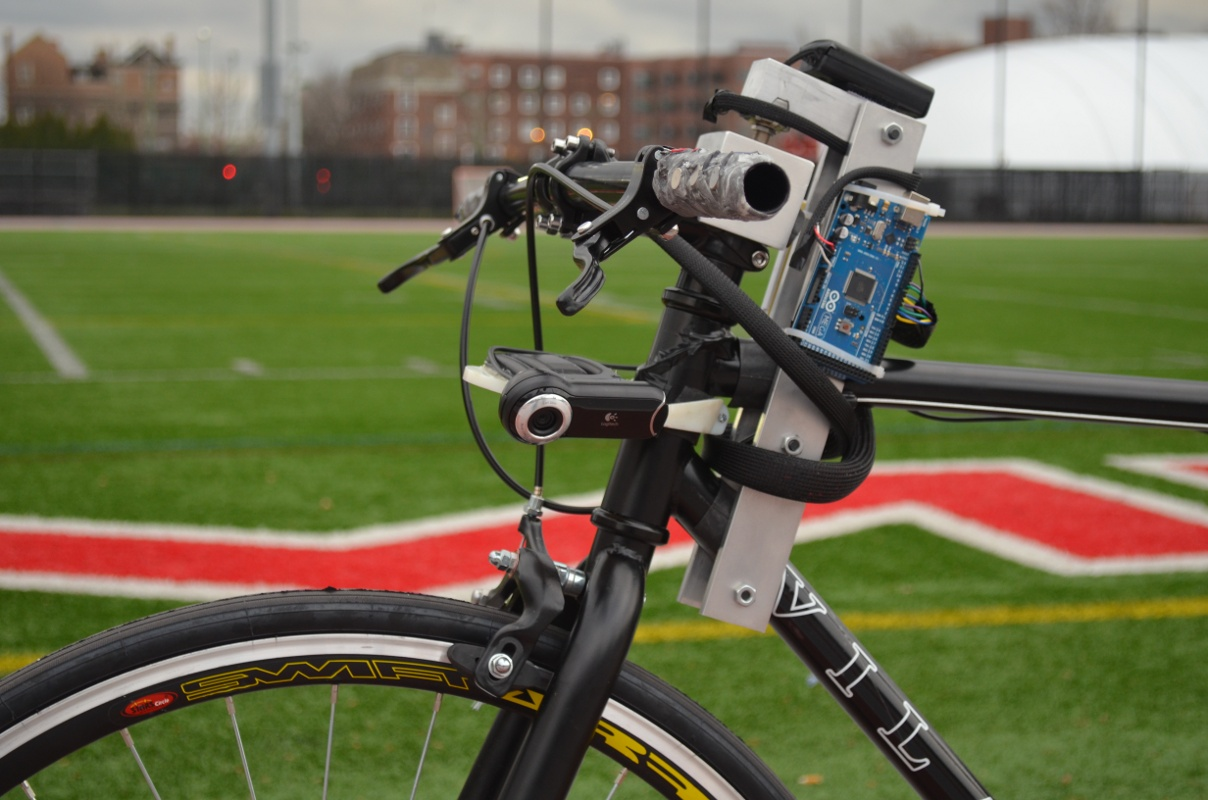
\includegraphics[scale=0.18]{blicycle_overall.jpg}
\caption{Main components of blicycle. The camera is used to localize the bike with respect to the track edge. Custom vibrating handlebars are controlled by a microcontroller and drive circuitry. The steering angle of the bicycle is also measured by a microcontroller and relayed to an onboard laptop in the rider's backback. This laptop processes all sensor data, generates a target desired steering angle for blicycle, and sends commands to the handlebar motors via the microcontroller.}
\label{fig:BlicycleOverview}
\end{figure}

\subsection{User Interface}
We chose to focus at first on the user interface portion of blicycle, or namely how to communicate when and how hard to turn. Any sort of visual interface was of course out of the question, and hence, with Brian's approval, we decided to focus on his sensing strengths: tactile and auditory interfaces.

We worked on two initial approaches in parallel: one auditory and one tactile. We envisioned an auditory interface using spatialized sound to lead the desired trajectory of the bicycle. By using Head-Related Transfer Functions (HRTF's), a concept borrowed from acoustics and signal processing, it would be theoretically possible to play sounds that appeared to come from different 3D locations around the head. We imagined using the superposition of multiple sounds - one to indicate a goal or turning direction, and others to indicate the relative bearings and distances to detected obstacles. In this way, a 3D soundscape would be constructed in realtime to inform Brian about the relevant world state as measured by blicycle's sensors. Towards this goal, we found an online HRTF database\footnote{We used the CIPIC HRTF Database from UC Davis: http://interface.cipic.ucdavis.edu/sound/hrtf.html} compatible with MATLAB that allowed us to play sound samples from specified directions.

\begin{figure}
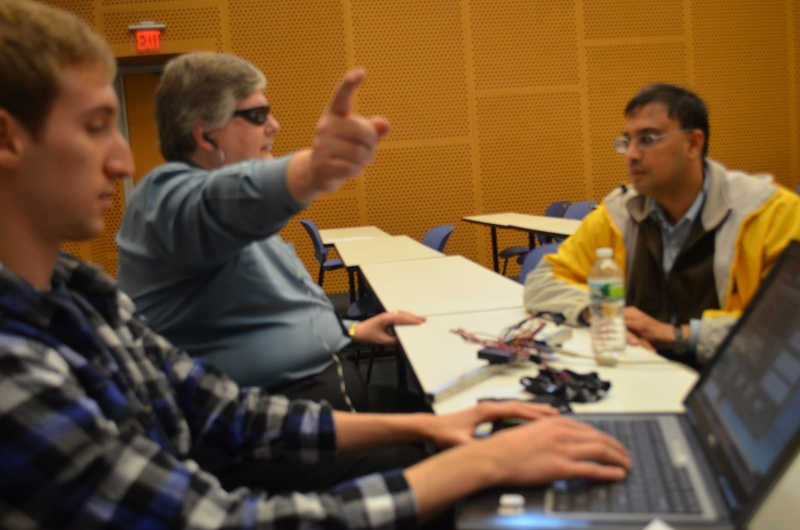
\includegraphics[scale=0.22]{spatial_audio.jpg}
\caption{Brian testing the spatial audio interface prototype. A sound was generated from a certain direction, played through headphones, and we asked Brian to point to its apparent source.}
\label{fig:SpatialAudio}
\end{figure}


Our second, parallel approach consisted of a pair of vibrating gloves. A small vibration motor (similar to what's inside a cellphone) was attached to each finger and actuated via PWM from a microcontroller. Our intent was that the location of the vibration (i.e., left/right hand, amd position within that hand) could communicate both the desired steering direction, and how hard to steer in that direction. This prototype can be seen in Figure  \ref{fig:VibratorGlove}.

\begin{figure}
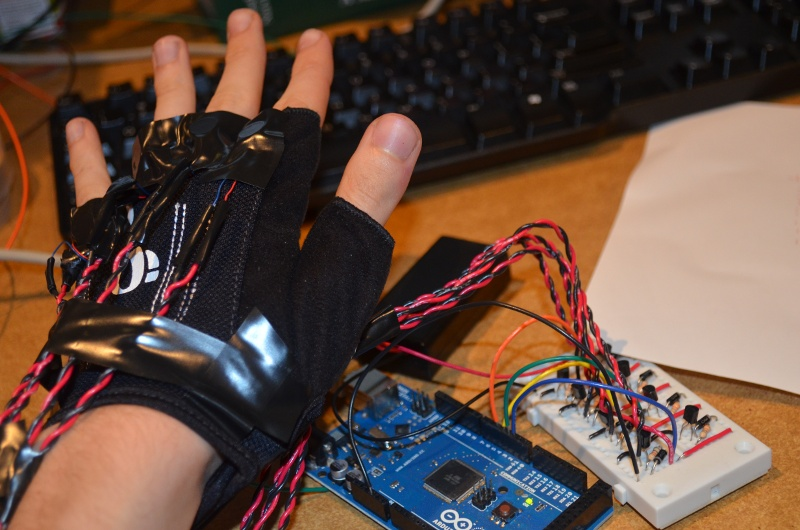
\includegraphics[scale=0.22]{glove_prototype.jpg}
\caption{Vibrating glove prototype. Each finger has a vibration motor and is individually controllable with PWM.}
\label{fig:VibratorGlove}
\end{figure}

\begin{figure}
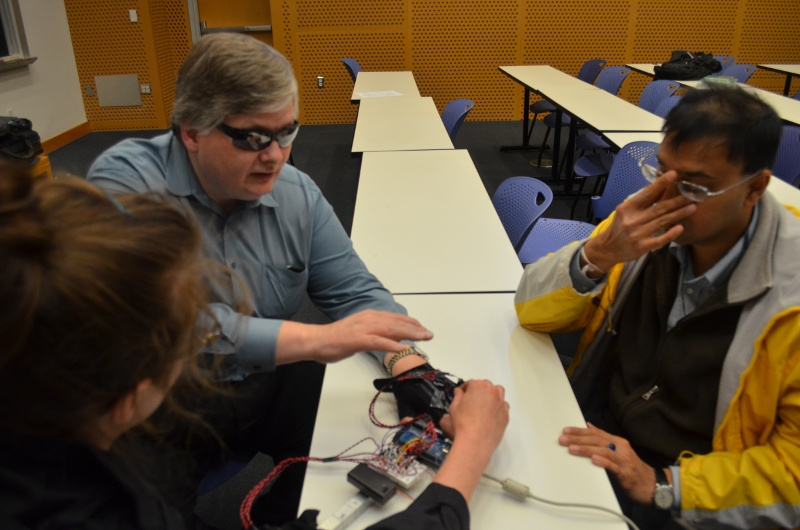
\includegraphics[scale=0.22]{brian_testing_gloves.jpg}
\caption{Brian testing the vibrating glove prototype.}
\label{fig:BrianTestingGloves}
\end{figure}

After developing these prototypes, we met with Brian to gauge his opinion. Figure \ref{fig:SpatialAudio} shows Brian testing the MATLAB spatialized audio interface, and Figure \ref{fig:BrianTestingGloves} shows Brian testing the vibrating gloves. Brian was able to tell the general direction of each of the spatialized sounds we played for him in our tests, however accuracy was not always precise. This can be attributed to the high sensitivity of HRTF's to recording conditions. Brian very much liked the vibration glove interface. We proposed several different control strategies, including a no vibration "sweet spot." For example, if the bicycle handlebar should be turned left, motors in the left hand would vibrate until the handlebar is turned to the desired position, at which time all vibration would stop. Should the rider overshoot and turn the handlebars too far, the right vibration motors would begin to vibrate. In this way, a control system is set up in which the desired position of the bicycle's handlebars can be communicated through vibration. Brian very much liked this interface and control strategy. He also liked the analog-like nature of having varying degrees of turn intensity, though the PWM was too hard to distinguish in the fingers. Brian preferred the tactile interface to the audio interface 9:1, so we decided to focus our efforts solely on the vibration interface from that point on.

Our next prototype sought to improve this design. Instead of using vibrating gloves, we decided to switch to vibrating handlebars. This design change was a result of considering the context in which Brian would be riding. Since the gloves were physically tethered to the bike via wiring, we were worried about Brian's safety should he need to remove his hands quickly from the bicycle. This would require either a quick disconnect cable, or a means of not tethering the user to the bicycle with wires. By using vibrating handlebars, all cabling could be routed internally inside the bike and the rider would be free to remove his or her hands hands at any time from the bicycle. Additionally, PWM on each motor was changed to binary on/off to make commands more distinguishable. One motor would always vibrate, and the more left or right it was along the hand indicated how sharply (left or right) the bicycle should be steered to reach the no-vibration sweet spot.

This handlebar prototype was tested with Brian using a software simulation of the bicycle (described in the "Simulator and Control Systems" section). We found that Brian was able to quickly turn to desired angles (within about 1-2 seconds) using the vibrating handlebars, and that this would likely be a feasible approach for the user interface.

\begin{figure}
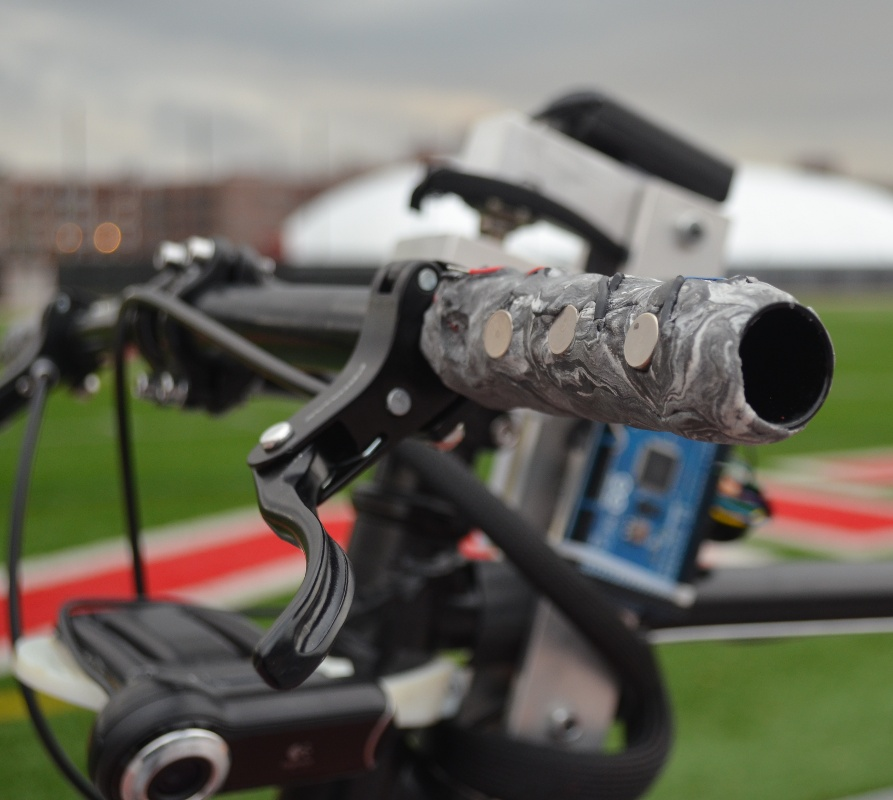
\includegraphics[scale=0.22]{vibrating_handlebars.jpg}
\caption{Vibrating handlebars. Note the metallic vibration motors attached via sugru to the forward side of the handlebars. Wiring is routed internally for aesthetics and safety.}
\label{fig:VibratingHandlebars}
\end{figure}

Our final prototype for the user interface was again a vibrating handlebar design, but now mounted onto the bicycle using sugru. Additionally, all cabling was routed internally throught he handlebar frame, providing a sleek and aesthetic design. However, one unforseen consequence of using sugru is that vibrations from left motors traveled all the way down the handlebar to the right side, and vice versa. This is because the sugru did not dampen out the vibrations enough, and hence fine-grained sensing was difficult because of the lack of vibrational isolation. In a future design, we would ensure that there is minimal cross-vibration on the handlebar. An image of the final vibration handlebar on the bicycle can be seen in Figure \ref{fig:VibratingHandlebars}.


\subsection{Obstacle Detection}
We did some experimentation with possible obstacle detection schemes while we developed the vibrating glove prototype. We investigated the use of a LIDAR, which would be capable of accurately finding nearby obstacles. However, the LIDAR scanner we had was heavy and required substantial power.

Shortly after, we decided to de-scope our project and not consider obstacle detection in this first spiral iteration. We made this choice due to time constraints on the other aspects of this project, specifically navigation and simulator development. Obstacle detection is of course a very important issue however, and will need to be properly addressed in any future iterations of this project.

\subsection{Navigation}
In this section, we'll discuss the navigation aspects of blicycle, or namely, how we determine the location of the bicycle to keep it on a desired trajectory. Our approach uses computer vision to localize the bicycle and a potentiometer to measure the steering angle. Once determined, this information about the bike position and current steering angle is sent to the controller module (discussed in the next section), which computes a desired steering angle for the bicycle and an appropriate vibration pattern for the handlebars. 

\begin{figure}
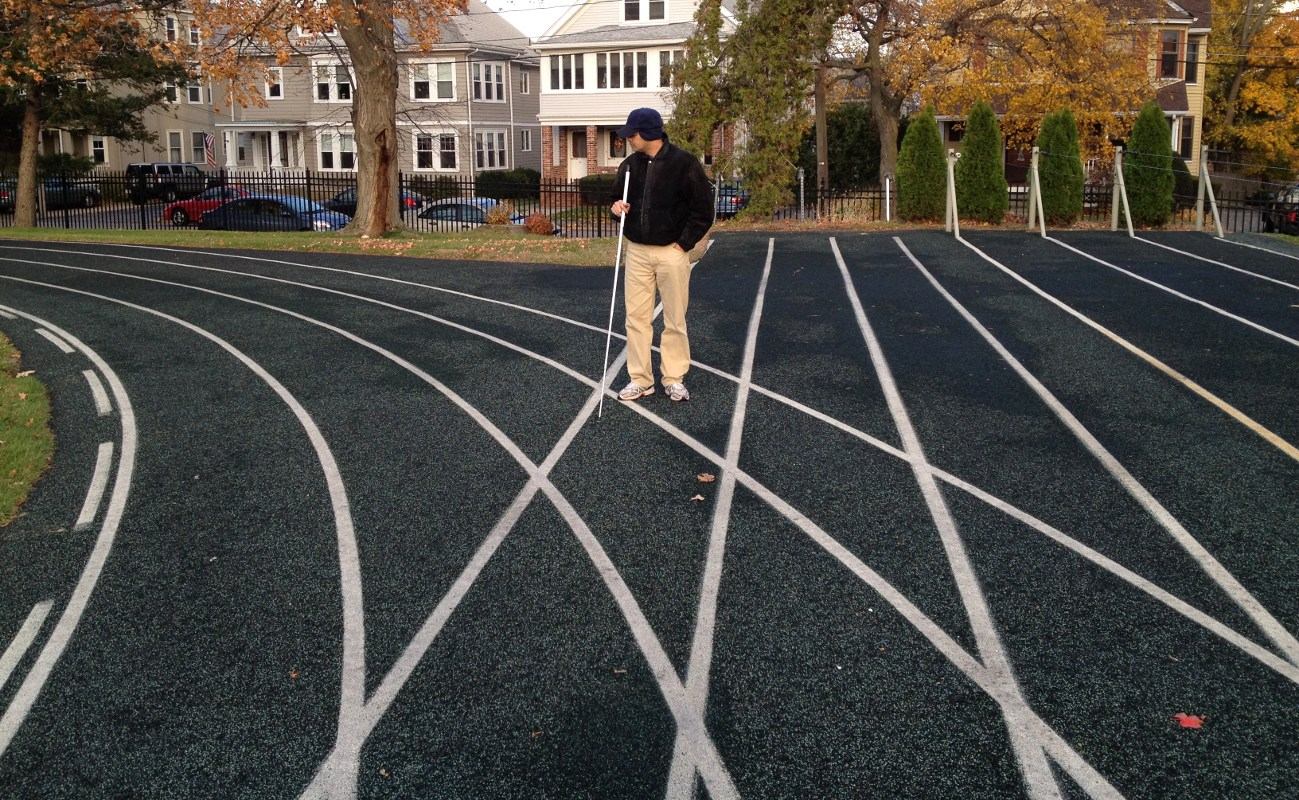
\includegraphics[scale=0.18]{track_curved_hash.jpg}
\caption{A curved, hashing pattern produced by normal lanes and merging starter lanes at the Perkins track. These pose a significant challenge for lane-tracking algorithms. Unfortunately, these problematic areas occur at the areas of highest rider danger along the track and hence motivated our decision to  use the inner grass / pavement border for computer vision instead of the white lanes.}
\label{fig:HashingPattern}
\end{figure}

Initially, we planned to use the white painted lanes on the track for guiding blicycle. The Perkins track where Brian will be riding has high-contrast lane markings that run parallel to the travel direction. However, a complication arose when we inspected the Perkins track in person. In addition to these normal lanes, there are also runner lanes that merge into these lanes and create a complex hashing pattern as shown in Figure \ref{fig:HashingPattern}. These patterns would be challenging for a computer vision algorithm to track robustly, and they unfortunately occur at the two most dangerous areas of the track. In the upper right corner of Figure \ref{fig:HashingPattern}, there is a steep hill, a metal pole, and a fence immediately after where the lanes merge - posing a significant danger should the lane tracking algorithm confuse the outgoing lanes with the normal lanes that curve around the track, and hence steer blicycle directly into an obstacle. Additionally, running along the outer edge of the track on one side are a collection of thick, waist-high metal guide cables used for straight races. These pose another significant hazard for a bicyclist on the Perkins track, so it is therefore desirable to keep the rider as far away as possible from the outer edge of the track. Therefore, again considering safety as a top priority given the context of this project and the riders functional abilities, we chose to use a computer vision algorithm that tracks the inner edge of the track instead of the lanes. This approach, in addition to side-stepping the issue of navigating a complex hashing pattern on the track, will also help keep the rider close to the inner edge of the track - away from the hazardous metallic guide cables running along the outer edge.

\begin{figure}
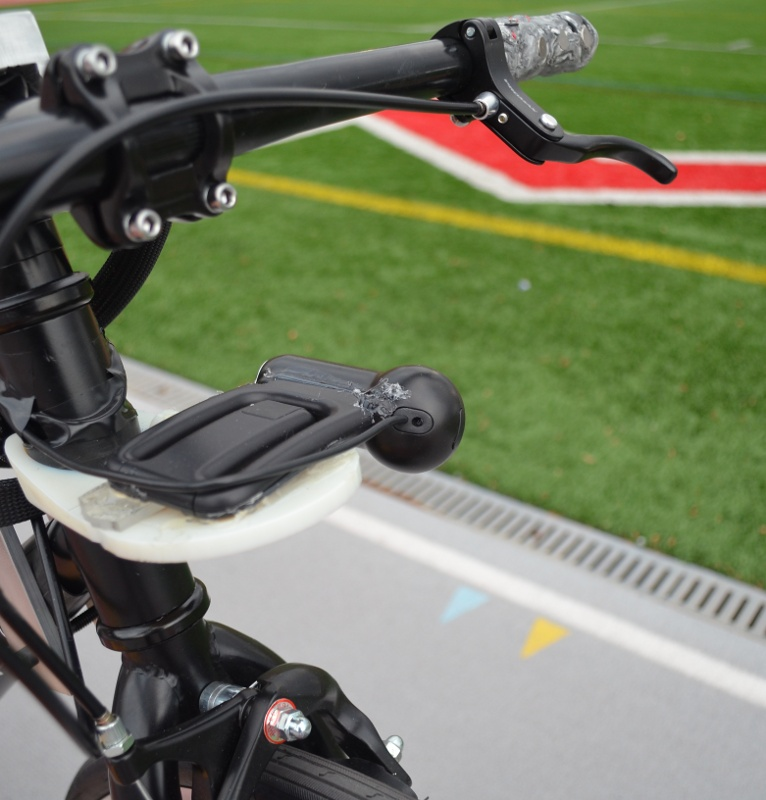
\includegraphics[scale=0.18]{camera_angle.jpg}
\caption{The sideways-facing camera monitors the track/pavement border.}
\label{fig:CameraAngle}
\end{figure}

\begin{figure}
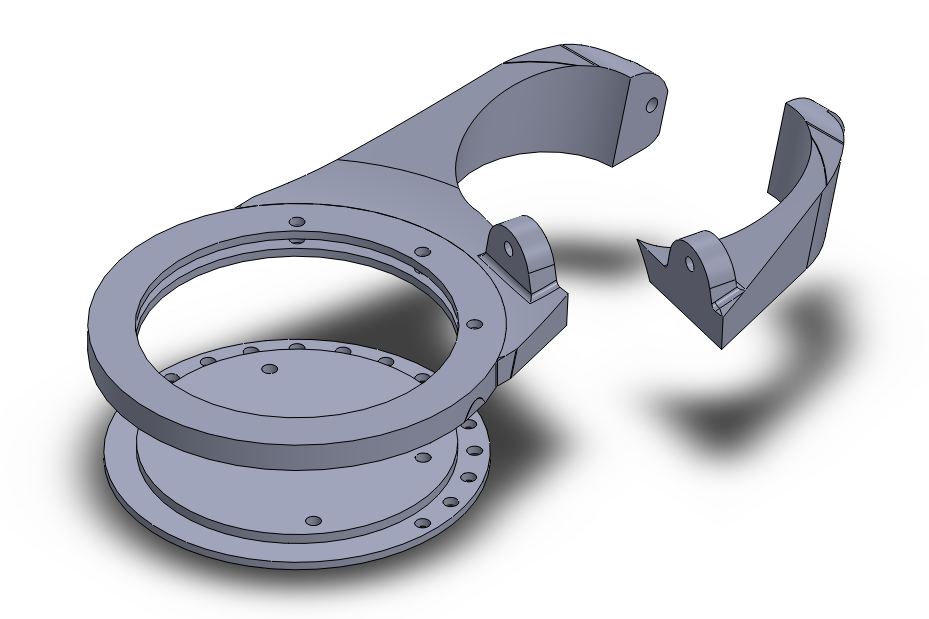
\includegraphics[scale=0.25]{camera_mount_exploded.png}
\caption{CAD model of custom camera mount.}
\label{fig:CameraMountCAD}
\end{figure}


We use a camera facing 90 degrees to the left when viewed from the rider's position, tilted slightly downwards, as shown in Figure \ref{fig:CameraAngle}. This allows the camera to face the track and monitor the grass / pavement edge. Mechanically, this required the design of a custom mount in order to attach the camera to the bicycle (see Figure \ref{fig:CameraMountCAD}. We originally considered many different camera mounting locations - such as on the handlebars facing down, offset from the bike centered over the track edge, etc. However, any approach in which the camera is significantly offset from the bike poses a danger from potential collisions with obstacles. As such, considering safety and the context in which the bicycle would be used, we chose to avoid any such mounting strategies.

\begin{figure}
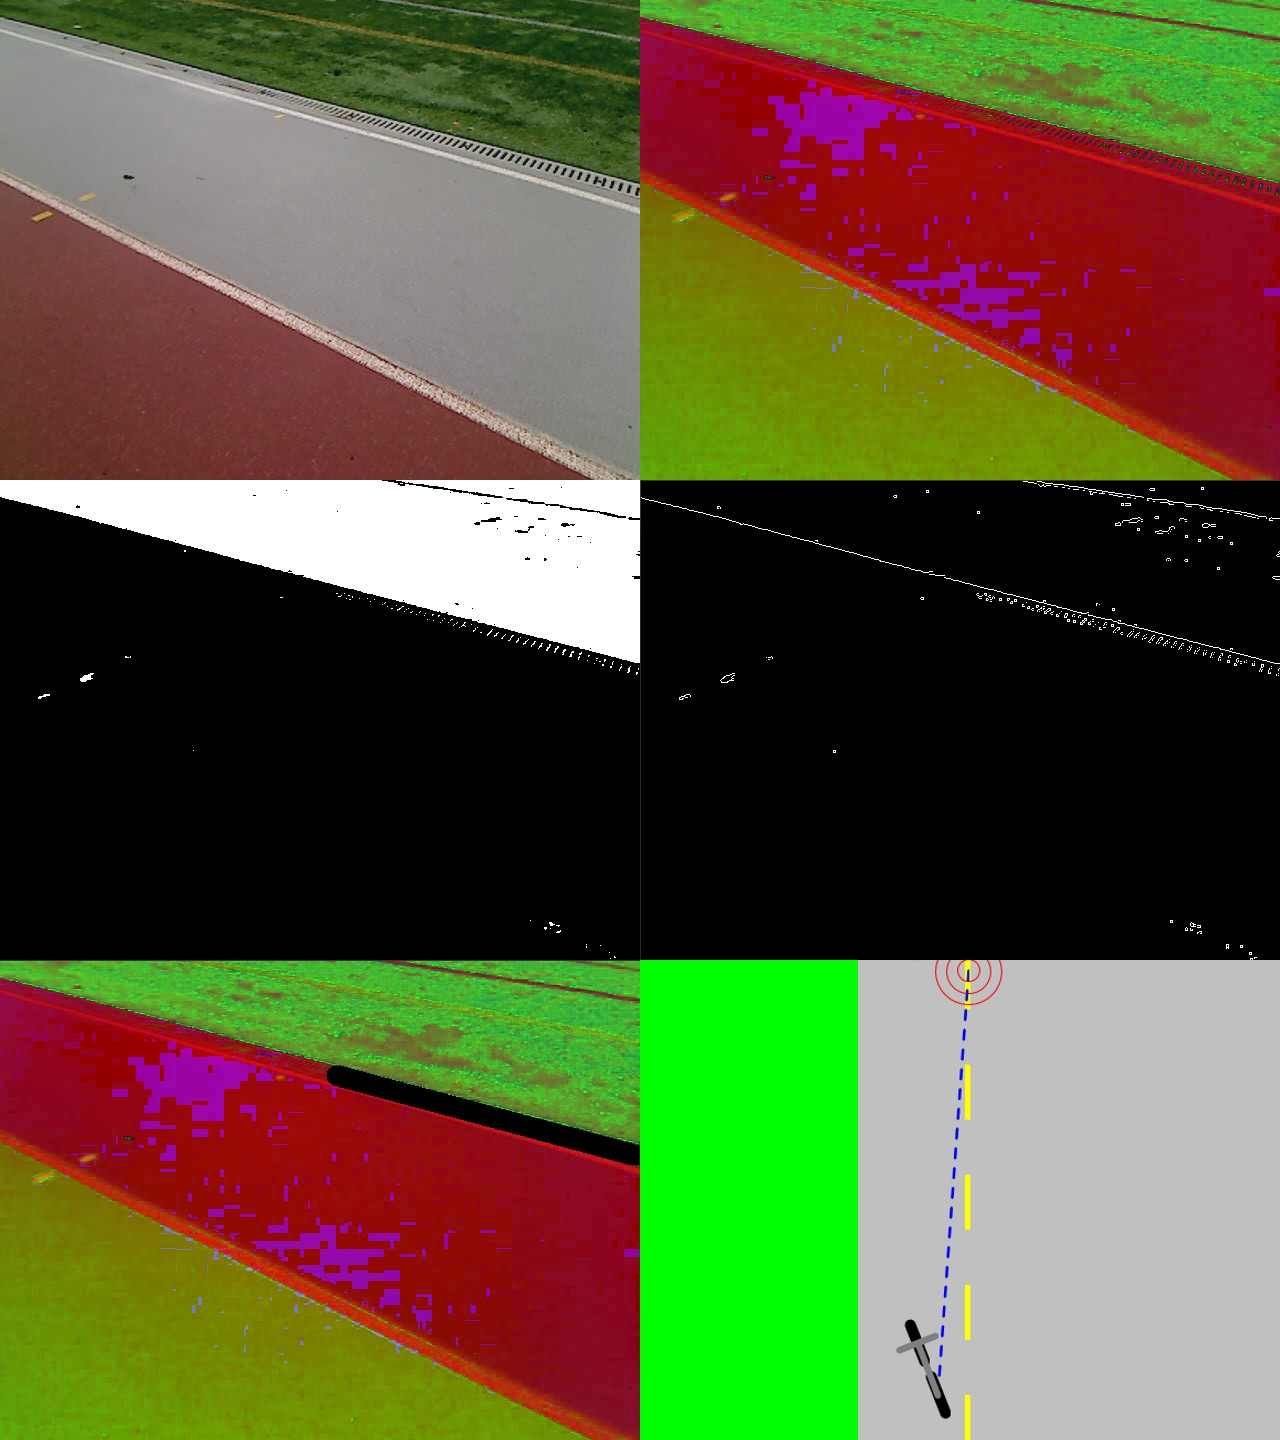
\includegraphics[scale=0.18]{cv_overview.jpg}
\caption{An example camera frame being processed by the computer vision algorithm. Flows from left to right, top to bottom: 1.) A frame is captured from the camera showing the track/pavement border. 2.) Conversion from RGB to HSV color space (shown here where B channel is H, G channel is S, etc.), 3.) Classifying each pixel as grass / nongrass by looking for pixels within a prespecified range of HSV values, 4.) Edge detection on the resulting binary image to highlight the grass-track border, 5.) Running a Hough transform algorithm on the edge-detected image to locate strong line segments in the edge-detected image. Each returned light segment is assigned a cost based on its position in the screen (lower coordinates favored) and distance from the last best line segment. The least-cost line segment (here shown in black) is chosen and outputted to the controller process, 6.) The controller/simulation process receives the line outputted by the CV module, and projects from camera space to the world frame using a table lookup on interpolated calibration data. The estimated position and orientation of the bicycle from the image is shown.}
\label{fig:CVOverview}
\end{figure}


The camera monitors the border between the green grass and pavement. By using a series of computer vision operations outlined in Figure \ref{fig:CVOverview}, a camera frame is processed to extract the edge of the grass. The output is a line segment connecting $(x_1, y_1)$ and $(x_2, y_2)$ points in the image, which is then converted to a $(\rho, \phi)$ format, denoting the distance and angle of the line with respect to a fixed point at the bottom-center of the screen. This transform has the property that all parallel line segments map to the same $(\rho, \phi)$, which is useful for tracking lines across images. The Hough transform used produces many line segments. We therefore assign a cost to each one based on the line's position in the screen (minimal $\rho$ favored) and distance to the last best line (favors "locked" tracking). This allows us to choose the line of lowest cost, which is used as the current estimate of the border. The computer vision module then transmits this $(\rho, \phi)$ line to the controller via a socket interface.

The next step is to convert $(\rho, \phi)$, which represent pixel-space coordinates, to $\Delta x$ and $\Delta \theta$ -the perpendicular distance from the bicycle to the track edge, and the angle of the bicycle's frame with respect to this edge, respectively. This is accomplished via a reverse lookup on training data. We recorded camera images at the track at a number of pre-measured $\Delta x$ and $\Delta \theta$ values. We then used MATLAB to interpolate between these points and reverse map them to the $(\rho, \phi)$ obtained from processing each image. This allows us to map from camera space to the world frame without explicitly modeling the camera (all computations lookup experimentally-measured data).

In addition to measuring $\Delta x$ and $\Delta \theta$, it is also critical to measure $\theta_{steer}$, or the steering angle of the bicycle. We accomplished this by mounting a potentiometer onto the handlebars of the bicycle such that the knob is turned whenever the handlebars are turned. We originally considered several approaches to measure the handlebar angles, including possibly using computer vision for this. This would involve attaching a fiducial or brightly colored object to the fork of the bicycle that would extend into the camera's view. As $\theta_{steer}$ is changed and the fork is rotated, this object would change position in the camera image, allowing $\theta_{steer}$ to be measured. We found however that, given our camera choice and mounting strategy of 90 degrees to the left, the object would need to protrude far out from the bicycle frame in order to be visible within our non wide-angle camera for the full range - this is something we wanted to avoid both for safety and aesthetic reasons. As such, we decided to use an approach involving a potentiometer mounted to the frame of the bicycle and to the handlebars to directly measure the angle without computer vision. While perhaps more complex mechanically, this design is safe, more reliably, and also simplifies the computer vision task.

A significant problem that must be addressed in any future iterations of blicycle is tilt when cornering. As blicycle tilts, the camera tilts too and hence detects a different line for the grass/track border. This theoretically and experimentally has manifested itself as inaccuracy of the position and orientation estimates when cornering. Possible ways to address this include the addition of an accelerometer and speedometer on blicycle to attempt to measure the tilt and compensate for it in software. An additional approach would be a mechanical solution in which the camera mount becomes an auto-leveling platform that keeps the camera always facing the same direction using gravity.

\subsection{Simulator and Control Systems}
Once the position and orientation of the bicycle with respect to the track ($\Delta x$ and $\Delta \theta$, respectively) have been estimated by the computer vision module, these are sent to the controller module, which runs as a separate process for safety (if the computer vision crashes, the controller will still run and can signal the rider to stop the bicycle safely).

\begin{figure}
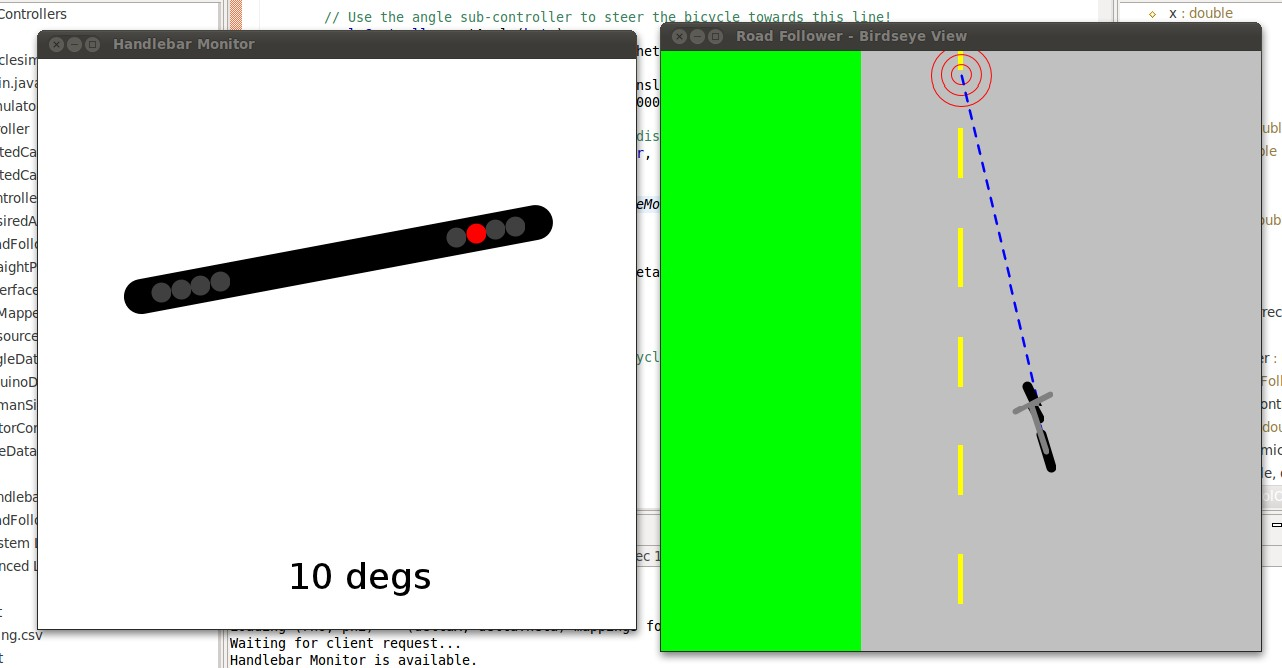
\includegraphics[scale=0.18]{simulator_screenshot.jpg}
\caption{A screenshot of the simulator interface. The left window shows the current measured steering angle of the handlebars and current vibration motor output. The right window shows the world state for the bicycle simulation.}
\label{fig:Simulator}
\end{figure}

Our controller module is tightly-coupled with a custom bicycle simulation engine we developed. This simulation was useful in testing a number of different control ideas we had, and was also used in user testing with Brian. Our simulation is capable of modeling a simplified version of bicycle dynamics: turning, radius of curvature, and decreasing velocity when turning are all represented. Additionally, the simulator is also capable of visualizing the world state. A screenshot of the simulator is shown in Figure \ref{fig:Simulator}.

When the vibrating handlebar prototype was being tested with Brian, this simulation was used to test various control ideas. Using a desired-angle controller that ignores bicycle dynamics and simply commands the handlebars to a desired angle through vibration using our no-vibration sweet spot approach, we were able to roughly measure Brian's response speed. We also tried a second control approach, which computed an error $e = k_1 \Delta x + k_2 \Delta \theta$ and used this signal to control the handlebars. While this approach does indeed favor going straight forward ($\Delta \theta = 0$) along the desired trajectory ($\Delta x = 0$), it was not stable. We found the system hard to control ourselves, and Brian often ended up going in circles in our simulation. The cause of this was that this control design does not consider $\theta_{steer}$, which is important in predicting the direction of the bicycle.

On our next iteration of control design, we instead used a forward-target controller. A point is computed along the desired trajectory forward of the bicycle's current position (shown as a red bullseye in Figure \ref{fig:Simulator}), and the bike is steered towards this angle using the desired angle controller. This controller felt intuitively much more stable and controllable than our first approach, though we were unable to test it with Brian. We further increased the accuracy of our controller by simulating the bicycle dynamics and future-predicting the bicycle's position approximately 1 second in advance, and using this as the input to the controller. This attempts to account for the rider delay in turning the steering wheel to the desired position.

\begin{figure}
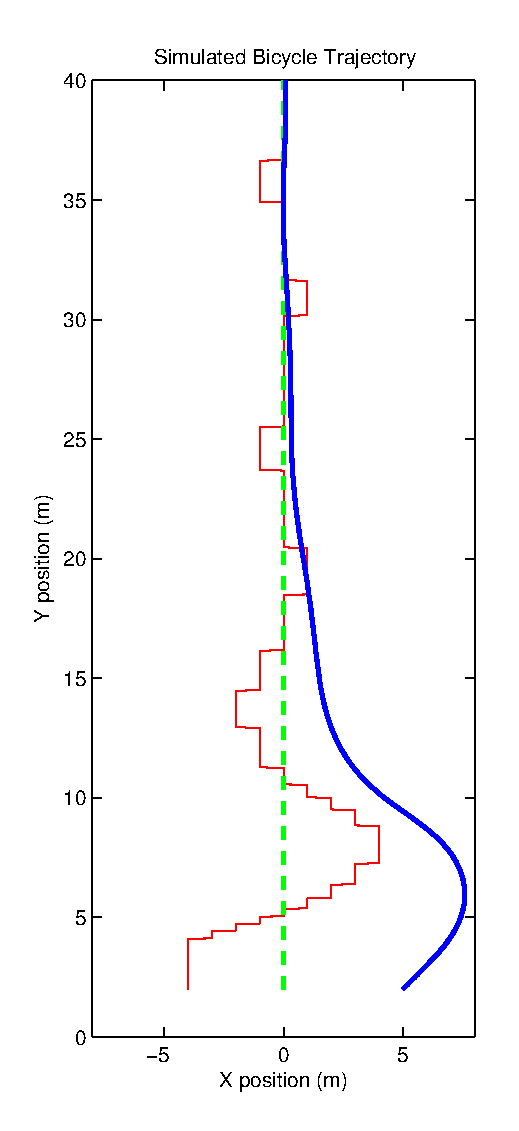
\includegraphics[scale=0.5]{stabilized-1-with-correction.pdf}
\caption{Simulation of the bicycle's trajectory. The bicycle, human operator with delay, and future target controller are all modeled. The blue curve represents the bicycle's trajectory (note that it starts in an offset position but is stabilized), the green dotted line represents the desired trajectory, and the red plot indicates the control signal sent to the handlebars (note that it slightly leads the trajectory due to the forward-predicting controller).}
\label{fig:ControllerStabilized}
\end{figure}

The simulator is also capable of modeling the vibrating handlebars and human rider with a delayed response time. With this, we were able to test the stability of our controller under different gains and forward prediction amounts. A resulting plot of controller stability for one such set of values is shown in Figure \ref{fig:ControllerStabilized}.


\section{Final Results}
By the end of the course, we were able to produce a functional prototype of bliycle. Although certainly rough around the edges and still requiring a great deal of work to become a final, polished product that is both safe and reliable enough to avoid abandonment, the various components of this project worked together in the end and, in our opinion, constituted useful design spirals in all design areas except obstacle avoidance. I was able to ride blicycle along a section of the MIT track successfully with my eyes closed, making turning corrections based only on the handlebar vibrations.

We wish we had done more user testing of our final prototype and control strategy with Brian, but were unfortunately unable to do so by the time of this paper's writing. As such, although we cannot formally evaluate our success metrics without Brian's opinion, we will estimate based on our own experiences and testing. Please see Figure \ref{fig:SuccessMetricsEval} for our estimated scores so far.

\begin{figure}
\begin{tabular}{| c | c |}
\hline
Success Metric & Estimated Score \\ \hline \hline
How aesthetic is the device? Conspicuous? & 7 \\ \hline
How comfortable is the device? & 7 \\ \hline
How safe does Brian feel with device? & 2 \\ \hline
How distracting / annoying is the device? & ?? \\ \hline \hline
How many laps can Brian complete? & ?? \\ \hline
How much time required to organize ride? & ?? \\ \hline
How many people required to be around? & ?? \\ \hline
How straight can Brian ride? Stays within \\ how many feet of center? & 15ft \\ \hline
How fast can Brian safely ride? & 10mph \\ \hline
\end{tabular}
\caption{Qualitative and quantitative success metrics.}
\label{fig:SuccessMetricsEval}
\end{figure}


In order to produce an assistive technology that our client would not abandon, much worked would be needed:
\begin{itemize}
\item Blicycle must be fully functional and reliable, as demonstrated from extensive user testing
\item Address obstacle detection
\item Address the cornering tilt issue present in computer vision
\item Address cross-vibration in handlebar design
\item Currently, the rider wears a laptop in his/her backpack. It would be significantly more convenient to have the netbook attached to the bicycle frame, and this would avoid annoying tethering issues.
\item The system must give alerts for low battery, and if any other error condition is detected (i.e., computer vision process crashes or doesn't have a lock on the grass/pavement border, etc.)
\item There is currently a separate battery pack for the vibration motors. It would be much more convenient in terms of maintenance to power the motors directly from netbook rather than have a separate battery pack. Brian would simply need to remove the netbook from the bicycle and charge it separately indoors.
\item The addition of sporadic audio alerts for high-priority information, or as a fallback in case vibrations fail
\item Make the system more weather-proof by encasing electronic components
\end{itemize}


\section{Reflection}

As the term proceeded, we learned more about Brian's preferences and intended use cases. For example, after our initial meeting, we had the impression that blicycle would have to be robust to many different types of environmental conditions - sunny weather, cloudy weather, snow, nighttime, etc. The road surface could potentially be affected by adverse weather conditions, and the computer vision is extremely sensitive to changes in lighting conditions. Additionally, in snowy weather, the grass may appear white instead of green. However, after further speaking with Brian, we realized that he did not intend to ride the bike in many of these conditions - he planned to ride in good weather, likely during the summer when it is still light outside. Therefore, after learning this, we were able to greatly simplify the complexity of our computer vision algorithms without compromising Brian's desired use case.

One aspect of this project that turned out to be easier than I expected was the camera calibration procedure. I had originally envisioned that it would be necessary to compute a camera transform to map pixel space coordinates into the world frame, and I expected that this would likely be quite complicated given the unknown optics and precise tilt of the camera. However, this turned out to be easier than expected using our approach of fitting to pre-measured calibration data.

One aspect of this project that turned out to be much harder than expected was getting good handlebar vibration performance. As we mentioned earlier, the left-right cross vibration that made it difficult sometimes to tell which vibration motors were being actuated. The metallic handlebars conduct all vibrations much more than we expected, and our choice of dampening materials didn't dampen the vibrations as much as we had expected. Therefore, getting good handlebar performance was something that we thought would be easy, especially given our initial prototypes, but this actually turned out to be quite tricky.

Thoughout the course of this project, we were able to apply many lessons learned from class to the design of our project. Perhaps the most significant of these is the need to design for the client's abilities - what he or she is good at it. In leveraging the client's functional abilities, it is possible to overcome many disabilities. We employed this approach in designing our handlebar user interface. Our client Brian has exceptional tactile sensing, so we designed an interface that would leverage this strength. An additional lesson that was quite interesting was learning about how easy it is for a product to be abandoned, and realizing that the quality required for assistive technology to be successful must be extremely high. While our current prototype is certainly not to this point, this lesson was key to understanding that we still have a lot of work to do on blicyce to decrease its chances of abandonment. A third interesting lesson was the one related to the ethics of user testing. Since we did user testing on Brian using our simulation software and handlebar prototype, it was interesting to hear about proper techniques for treating subjects. For example, making it clear that the technology is being tested - and not the individual - was very interesting and relevant to our project.

Here are each team member's individual contribution to this project:

Steve:
\begin{itemize}
\item Electronics design for vibration gloves/handlebars
\item Microcontroller firmware
\item Simulator software and GUI visualization
\item Controller design ideas and software implementation
\item Computer vision and navigation 
\item Fabricated potentiometer mount (designed by Emily), final assembly/wiring of bicycle
\item Outdoor tests with bicycle at MIT track
\item Experimentation with: spatialized audio, LIDARs, alternate cameras
\end{itemize}

Emily:
\begin{itemize}
\item Mechanical design of vibration gloves
\item Designed, constructed the physical handlebar mockup for simulator
\item Indoor user testing of simulation and handlebar mockup with Brian
\item Mechanical design and fabrication of final vibrating handlebars 
\item Design and fabrication of camera mount
\item Design of potentiometer mount
\item Controller design ideas
\end{itemize}

Sunish:
\begin{itemize}
\item Team advisor - gave general advice on all aspects of project
\item Provided knowledge about technologies in blind community
\item Visits with Brian 
\item Analysis of Perkins track
\end{itemize}

Personally, I can honestly say that I very much enjoyed working on this project. Not only was it a great technical challenge from which I learned a lot (computer vision, OpenCV, approaches to designing for people with disabilities), but it also hit quite close to home for me. As an avid bicyclist, one of the things that I would likely miss very much if I were to go blind today would be my ability to ride a bicycle. I therefore hope that our work this semester, which by no means solves this problem in its entirety, does however take useful first steps towards making the world more accessible and letting people with disabilities pursue some of the hobbies and pastimes that they most enjoy.

\end{document}